\section{The boundary}\label{sec:boundary}

\paragraph{The question.}
The structure of the previous sections holds on the inputs of Table~\ref{tab:inputs}, and it fixes no number. The principle asks for more than structure: it would have to single
out a world. This section asks how far the same structure reaches toward the Standard Model's flavour numbers, and
where it stops. We answer with results of one kind, each stated with its frame and its grade: what the weave's
symmetry, its clock, its frames and its motion do \emph{not} fix. The results are labelled N1--N7. Four of them (N4--N7) are sealed negatives, a compiled verdict, or sealed
scoreboards. The one-Higgs census (N5) tests a model of the program's own (one Higgs, $\tau=\omega$, eighteen flat lines),
so it locates the boundary of the program and not of the grammar. All of them are kept in the paper, because a boundary located only by success would not be located. The
program's arcs are cited by number (B1604 and so on) as the record, not as papers~\cite{OriginAxiomRepo}. No result
below is a value of the Standard Model (0 of 19).

\paragraph{The spine.}
A law of invariance fixes an orbit, not a point of it: a selector that commutes with a group acting on the possible
numbers cannot choose among the points of one orbit (the record's orbit-to-point gap, B990, stated there for orbits of
pairs of $27$s).
At a point of the fibre the residue coupling has rank one and the coupling has rank at most two for every flat line
(B1653); at the symmetric point $\tau=\omega$ the Higgs's symmetric vacua give masses $(1,1,0)$, a rank-one coupling, or a
hierarchy set by the two defects (B1657), and the isotropic vacua carry no hierarchy of their own. Hence whatever chooses the numbers is not given by the
symmetry alone, although it acts at one. N1--N4 below are the symmetry side of this statement; N5--N7 are the
quantitative side, on the matter and the motion.

\subsection{No index on a thread}

\begin{lemma}[N1; B1604]\label{bd:noindex}
Let $N$ be the interior of a compact $3$-manifold with torus boundary (a cusped hyperbolic $3$-manifold, or a finite
cover of one), and let $E$ be any flat module. Then
\[
  \chi(N;E)=\chi(N,\partial N;E)=\operatorname{rank}(E)\,\chi(N)=0,
\]
because $\chi(N)=\tfrac12\chi(\partial N)=0$: the double $N\cup_{\partial N}N$ is a closed odd-dimensional manifold, so
$0=2\chi(N)-\chi(\partial N)$, and $\chi(\partial N)=0$ for a torus. By Poincar\'e--Lefschetz duality $h^2(N;E)=\dim H^1(N,\partial N;E^*)$ and
$h^3(N;E)=0$. The class index $I(E)=n(E)-n(E^*)$, where $n(E)$ is the dimension of the interior cohomology, the image of
$H^1(N,\partial N;E)\to H^1(N;E)$, and $n(E^*)$ equals, by duality, the interior dimension of $E$ in degree two, is therefore not an Euler characteristic, and no
index theorem of Euler type computes it.
\end{lemma}

\emph{Scope.} This is standard topology (the vanishing of $\chi$ on odd-dimensional manifolds, and duality) applied to
the record's class index; the application is the arc's. The consequence is the one we use: a generation count obtained
as a flat-module index on a thread, or on a cover of one, is not given by an Euler-type index theorem; this argument does not exclude other index constructions. The
record also finds, by computation on the modules it checked, that $I(\Lambda^2E)$ is not a function of $I(E)$ (B1603). A
physical count needs an even-dimensional object with a non-flat bundle, or else ``a generation'' means a sector
selected by a character, which is a selection. This is why the chiral three of Section~\ref{sec:three} is stated with
three inputs and a reading, and not as a consequence of the thread alone.

\subsection{Residual symmetries against the data}

\begin{theorem}[N2; B1620, B1625]\label{bd:reducesnone}
Let $G$ be the weave's group (the lifts of $L$ and $R$ on $V=T\oplus\bar T$; order $96$, faithful and irreducible on the
triplet $T$). Take every subgroup $H\le G$ ($68$ subgroups in $26$ classes) as the residual symmetry of one sector, none
chosen.
\begin{enumerate}
\item A sector has three distinct masses exactly when $T|_H$ is a sum of three characters, that is when $H$ is abelian ($57$
  of the $68$), and every such residual leaves the masses free.
\item For every ordered pair of such residuals the family of mixing matrices has dimension $0,1,2,3$ or $4$ (the rank of
  the map to the nine $|V_{ij}|^2$ and the Jarlskog invariant), and no family of dimension below $4$ reaches the CKM
  matrix at $3\sigma$.
\item This holds with the mass term in $\bar T\otimes T$, in $T\otimes T$ and in $\mathrm{Sym}^2T$ (with $57$, $24$ and
  $16$ viable subgroups), and in every frame on record where the inner automorphisms act.
\end{enumerate}
\end{theorem}

\emph{Scope.} Proved by exhaustive computation over the subgroups and the three tensors; the block test used for the
CKM bound is necessary and sample-free, while the reach of the PMNS matrix is decided by a fit (and was regraded with
a strict predicate in B1625, the minimum unchanged). The statement is scoped, as the record scopes it, to the frames
where the inner automorphisms act; on the ruled branch the count is a lower bound under the modular-flavour ansatz. For
couplings in the modulus $\tau$ alone, the inner automorphisms generate an abelian group of order four that splits $T$
into three lines with distinct characters, so every mixing is a permutation (B1620). The statement is of a known kind. Scans
of the residual symmetries of finite groups find, in the settings they consider, quark mixing at leading order that gives
the Cabibbo angle and not the full CKM matrix~\cite{HolthausenLim2013,YaoDing2015}. The result here is the same answer for
this particular group, computed on all its subgroups; we are not aware of a published discrete-flavour model that
reduces the thirteen by a definite number~\cite{Feruglio2019,NovichkovPenedoPetcov2021}.\footnote{A fourth boundary statement, a count of the
parameters that one-modulus modular fits need (B1637), is not stated here. Its near-cusp fits were artifacts of the
evaluator's precision, and its re-run on an accurate evaluator is owed.}

\subsection{The clock stays in the grading}

\begin{theorem}[N3; B1621, B1633]\label{bd:clock}
Let the clock be the parity class $(A_n,B_n)$ modulo $2$ of the rule's fixed-point word, acting on $T$ as conjugation
by the word's prefix, which is $\mathrm{diag}(\chi_p)$ on $T$.
\begin{enumerate}
\item The clock's matrices span exactly the diagonal algebra. Every coupling that reads the clock is diagonal in the
  parity lines under every tensor: it splits masses and never mixes, and its invariant mean on $T$ is zero.
\item The tick $\sigma^2=LR$ acts on $T$ with eigenvalues $\{1,\omega,\omega^2\}$ and cycles the parity lines. Its
  operator mean is the rank-one democratic matrix, which does not commute with the clock, and its means on the clock's
  forms give three equal masses under all three tensors.
\item The averaged word coupling is a scalar on $T$ (B1633).
\end{enumerate}
\end{theorem}

\emph{Scope.} Exact up to floating point, with the word taken to $F_{30}$. The democratic matrix is classical; the
statement that it is a mean and not a commutant leaves the earlier refutation of $\mathbb Z/3$-forced democracy untouched.
The consequence is that the principle's own data (its clock and its tick) fix no number: they supply a grading and a
scalar.

\subsection{The frame tribunal}

The same computation gave different answers in different frames: the first-generation zero holds in one and dies in
another, and ``the Higgs in $M$'' is the electroweak Higgs in one frame and a flavon in another. A value can be
derived only along a chain with no hidden choice, and the frame is the first link of every chain, so the frames were
judged before further numbers were chased.

\begin{verdict}[N4; B1652]\label{bd:tribunal}
Take the frames on record (F1, the fibre at one $\tau$; F2, the surface frame with $\tau$ integrated; F3, an E$_8$
frame studied within the program; F4, the thread frame) and the eight demands D1--D8: the moves act as symmetries; the chiral
three; an anomaly-free hypercharge; an electroweak Higgs that couples the matter; a possible hierarchy; no free number
beyond the tagged postulates; CP violation possible; the scale and gravity. Then no frame on record is shown to
satisfy the demands on its own. The parent that would satisfy all of them is a seven-clause specification, and it is a
conjecture.
\end{verdict}

\emph{Scope.} A compiled verdict on the record's evidence of 2026-10-14, with each cell graded and cited. ``Shown''
means shown by a computation reproduced in the record; cells resting on an unreproduced computation are read and not
built on, and the
verdict needs only the verified failures and the untested cells. Representative cells, not the table:
F1 holds the chiral three given the triplet postulate and allows CP violation, but its hierarchy needs a free number
per sector and its D1 holds only given a vacuum that no dynamics on record selects; F2 holds the moves but needs a
source from outside the weave for the three and forbids CP violation; F3 holds the moves only by a supplied completion
that, on its flat background, loses the weak roots and the hypercharge, and its physical index is not computed. A
further candidate, formed inside the program, was refuted by the record (it fails D2 and D4 on the data) and is not
counted. The scope note on F3 applies: the table is evidence that no exhibited frame discharges every demand,
not that every frame fails.

\subsection{One Higgs against the data: a scoreboard}

\begin{scoreboard}[N5; B1660; negative as sealed]\label{bd:census}
On none of the eighteen admissible lines at the symmetric point $\tau=\omega$, in none of three readings of the up
sector (the same coupling $S$, the coupling $\tilde S=\epsilon\bar S\epsilon^{T}$, and the conjugate $\bar S$), does a single Higgs reproduce the data's five
non-electron mass ratios: no fit was found below the conservative bound $\chi^2=11.07$ (the $95\%$ point of $\chi^2$
with five degrees of freedom; the minimum over the fit's parameters is at most the value at the true point, so the bound
is one-sided and conservative), and the best was $34.40$ (the
conjugate reading on the pair of lines $(p_1,p_2)=(1/9,7/9)$ and $(8/9,2/9)$, with $w=p_1\tau-p_2$).
\end{scoreboard}

\emph{Scope.} A scoreboard, not a blind test: the data~\cite{HuangZhou2021} were seen. The census is for the canonical
end condition and the twisted frame of Section~\ref{sec:couplings}, at $\tau=\omega$, and the search was shown to recover
planted worlds in the data's regime. The end radius was a free parameter of the fit, over a domain
($2\pi\mathcal E+c_s>0.5$ in every channel, unbounded above) that contains both canonical radii at $\omega$ (Census
law~\ref{cl:cusp}: $0.692$ and $2.786$), so the canonical radii are among the values the fit could take. Its starts had
$\mathcal E\ge2.5$, and the lift with the exact norms outside a horoball differs from B1654's form by 17 to 25 per cent
(B1667). The end radius is a free parameter of the search, so the best value found bounds the best fit from above only. The census therefore does not by itself certify the result at a fixed radius, such as the canonical cuts of Census law~\ref{cl:cusp}. The misses are the two middle ratios, $m_s/m_b$ too large and $m_\mu/m_\tau$ too
small. The data put $(m_\mu/m_\tau)/(m_s/m_b)$ at $3.14$ ($2.9$ to $3.4$ within the strange-quark mass's uncertainty
alone)~\cite{HuangZhou2021}, against $0.63$--$1.75$ at the best points of the census
(Figure~\ref{fig:census}); the up quarks' $m_1/m_3$ is met. The Georgi--Jarlskog relation between the down quarks' and
the leptons' middle masses~\cite{GeorgiJarlskog1979} is context, not a claim.

Two post-seal explorations bound what the negative means, and both are labelled as explorations. First, there is no
ceiling: with no other target, the ratio $(m_\mu/m_\tau)/(m_s/m_b)$ reaches between $9$ and $34$ over every Higgs and
every end radius on four lines, so the misfit is a joint conflict among the five targets and not a bound on one of them.
Second, without the up quarks the down and lepton targets fit exactly. A second Higgs for the up quarks therefore makes
the ratios fittable, which is why it needs a blind test and not a further scoreboard.

\begin{figure}[t]
\centering
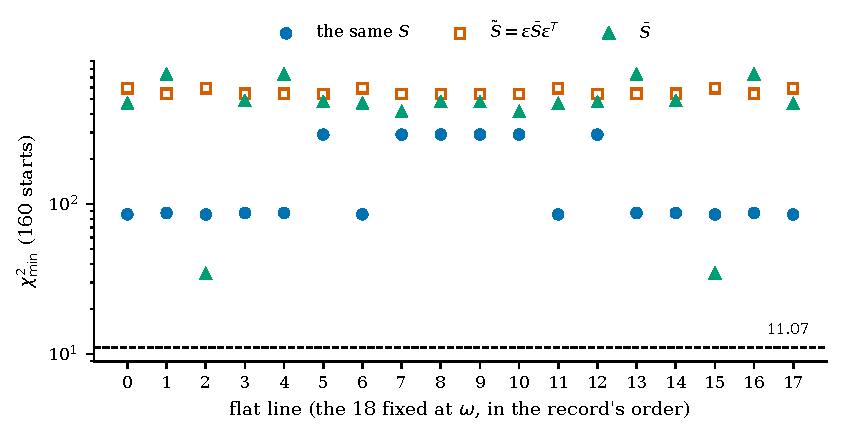
\includegraphics[width=\linewidth]{figures/fig_census}
\caption{B1660's scoreboard. The best $\chi^2$ (160 starts) on each of the eighteen admissible lines in each of three
readings of the up sector, against the conservative bound $11.07$. Scope: one Higgs at
$\tau=\omega$ on the admissible lines, the data seen; a scoreboard, not a ceiling, and not a statement about two Higgs
fields.}\label{fig:census}
\end{figure}

\subsection{The pull-back's strength}

The grammar's states move: a walk of steps and their pull-backs escapes at a positive rate whatever the pull-back's
strength (for the symmetric walk by Kesten~\cite{Kesten1959} and Furstenberg~\cite{Furstenberg1963}; for the other weights
by the same theorem of Furstenberg, as the support generates $\SL(2,\Z)$; the rates are measured here). We call the pull-back's weight $p$ (the probability of choosing a pull-back
at each step). The question is which quantities the weight $p$ sets.

\begin{censuslaw}[N6; B1663; negative as sealed]\label{bd:strength}
For $p=0,0.1,\dots,0.5$ the walk on $L,R,L^{-1},R^{-1}$ (equal weights within each pair) has the following behavior.
\begin{enumerate}
\item The probability that the end lies on the positive side falls from $1.000$ at $p=0$ to $0.531\pm0.028$ at
  $p=\tfrac12$ ($\tfrac12$ exactly there, by the mirror).
\item The escape rate falls from $0.3959\pm0.0004$ per step at $p=0$ to $0.1007\pm0.0005$ at $p=\tfrac12$. The escape rate
  is $(1/n)\log\|X_n\|_F$ at the first $n$ at which an entry of the walk's product $X_n$ exceeds $10^{60}$ (or at
  $n=40\,000$), an estimate of the top Lyapunov exponent, which is half the hyperbolic drift of $d(i,X_n i)$. This
  first-passage estimator differs from a fixed-length estimate by about $0.1\%$ at $p=0$ (low) and about $2\%$ at
  $p=\tfrac12$ (high): the fixed-length estimate gives $0.3964\pm0.0001$ and
  $0.0987\pm0.0002$ (\texttt{checks/lyapunov\_fixed.py}; B1662 reports $0.0992$ at $p=\tfrac12$).
\item The motion's averaged defect $\langle f\rangle$ is $0.5157\pm0.0012$ at $p=0$ and $0.5178\pm0.0013$ at
  $p=\tfrac12$; over all six values of $p$ it varies by $0.0028$. The preregistered prediction that it would differ by
  more than five standard errors failed.
\end{enumerate}
\end{censuslaw}

\emph{Scope.} The statement is for $L$, $R$ and their inverses with equal weights within each pair, with resolution about
$0.009$: a mild dependence of that size is not excluded. The averaged defect is a definite number, $0.517$, the forward
motion's; it differs from $0.31500491$, the average of $f$ over the modular surface, which is the value along a typical geodesic
(the \emph{typical motion's} value), and no dictionary attaches it to a mass. The strength $p$
sets the side and the speed. It does not set the defect, so the pull-back adds no number to the sizes.

A post-seal exploration, labelled, bears on why. The continued-fraction digits of the limit follow the geometric law
$2^{-k}$ at $p=0$ and at $p=\tfrac12$ alike (frequencies $0.502,0.248,0.123,0.064$ and $0.504,0.253,0.121,0.060$ for the
digits $1$ to $4$, on $24\,000$ digits each), against the Gauss--Kuzmin law $0.415,0.170,0.093,0.059$ of a typical point.
At $p=0$ the geometric law is exact and classical: the steps are fair independent letters, the digits are their run
lengths, and the limit's law is Minkowski's measure $d{?}(x)$, which is singular~\cite{Denjoy1938,Salem1943}. The $p=0$
reading is therefore a control. At $p=\tfrac12$ the same law is a reading of $24\,000$ digits and not a proof. For
$p>0$ the steps generate the group, and the exit law of a finitely supported generating walk is singular: for
$\SL(2,\Z)$ by~\cite{GuivarchLeJan1993}, and for nonuniform lattices in general by~\cite{GadreMaherTiozzo2015}. We use
neither statement beyond that scope.

\begin{figure}[t]
\centering
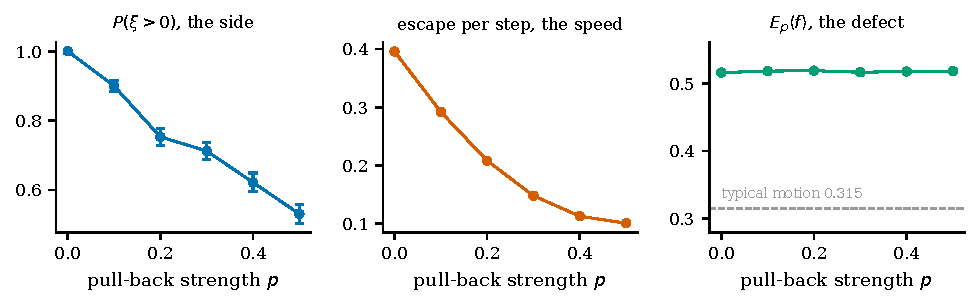
\includegraphics[width=\linewidth]{figures/fig_pullback}
\caption{B1663. (a) The side $P(\xi>0)$, (b) the escape rate and (c) the averaged defect $\langle f\rangle$ against the
pull-back weight $p$, with the typical motion's $0.31500491$ marked. Scope: the walk on $L^{\pm1},R^{\pm1}$ with equal
weights within each pair; the flat panel (c) is the negative result, and its resolution is about $0.009$.}\label{fig:pullback}
\end{figure}

\subsection{The layers}

The weave has two sides, the sum over closed geodesics (the threads) and the spectrum of the modular surface (the waves).
We asked what the threads' layers do on the program's own quantity, the matter's defect $D$ with $f=|D|/\|\rho\|^2$. The
sequence of arcs is part of the result. B1664 and B1665 were sealed and failed their own gate at the two zeros of $D$
(Section~\ref{sec:methods}); both are recorded as inconclusive. B1666 re-sealed the test with an estimator that no
zero can spoil; its cells hold, and it is a sealed scoreboard, because the read-outs of the first two were seen.

The period phase is Theorem~\ref{thm:phase}, which holds for every thread (checked to trace $600$,
Census law~\ref{cl:phase}): a coherent average of the amplitude survives only on the quarter of threads with
$\#L\equiv\#R\pmod4$. The layers then give the following.

\begin{scoreboard}[N7; B1664--B1666]\label{bd:layers}
To trace $600$, and on the threads of that range:
\begin{enumerate}
\item the layer averages of $f$ by trace approach the typical motion's $0.31500491$ (the top quarter of the traces, $451$ to
  $600$, gives $0.3144$, against $0.3692$ for traces at most $20$), with the distance falling as
  $t^{-0.51\pm0.05}$;
\item the phase-one coherence of the amplitude falls with length, with slope $-0.269\pm0.083$. The \emph{coherence} of a
  thread is $\bigl|\int\psi\,ds\bigr|/\int|\psi|\,ds$ over one period, and the phase-one threads are those whose period
  phase is $1$. The slope is $3.2$ standard errors from $0$ and $2.8$ from the random-phase value $-\tfrac12$, the error being
  an ordinary least-squares error over threads treated as independent;
\item the normalised coherence of the cusp family $L^{4m+1}R$, after a first drop, climbs toward one ($0.637$ at $LR$, then
  $0.285,0.717,0.861,0.919,0.948,\dots,0.99994$), and the most coherent phase-one thread is the longest of the family.
  The root $LR$ is not singled out. This is a read-out with no criterion, and the size of the coherent amplitude is not
  compared.
\end{enumerate}
\end{scoreboard}

\emph{Scope.} Item~1 is the trace formula's constant mode on the program's own quantity, expected from the
equidistribution of closed geodesics on the modular surface and of their discriminant layers~\cite{Duke1988,Sarnak1982}, with cycle integrals as in~\cite{KatokSarnak1993}; it is a check of the weave side against
the wave side, not a new equidistribution theorem. The law of the phase is a sealed identity; items~1--3 are a
scoreboard (the earlier read-outs were seen). What it does not show: the physical amplitude (this is $D$ alone, and the
physical amplitude needs the Higgs's own law), any Standard Model value, or the rate of approach as a law. The approach to the constant mode is a property of bounded
quantities such as $f$; it is not claimed for quantities that grow at the cusp.

\begin{figure}[t]
\centering
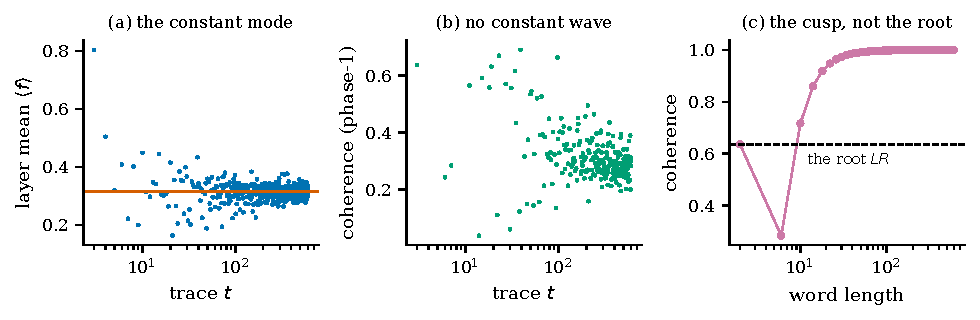
\includegraphics[width=\linewidth]{figures/fig_layers}
\caption{B1666. (a) The layer averages of $f$ against the trace $t$, approaching the constant $0.31500491$. (b) The
layer mean of the phase-one coherence against the trace $t$. (c) The cusp family $L^{4m+1}R$ against word length, with
the root $LR$ marked. Scope: traces at
most $600$, $30\,674$ threads, and the matter's defect $D$ alone; a scoreboard.}\label{fig:layers}
\end{figure}

\reading{The boundary has a shape. What the weave's symmetry, its clock and its frames fix is the structure and none of
the numbers, and each attempt to let a motion choose the numbers returns a constant: the pull-back's strength changes
the speed and not the size; the threads' averages return the surface's own constant; and the one place the motion
prefers something (the coherent rule) it prefers the cusp, where the defect vanishes. This is a reading of
Sections~\ref{sec:boundary} and~\ref{sec:selection} together, and it states no result.}
